\begin{frame}{The \tHq lepditau channel}
  \begin{columns}
    \begin{column}{0.5\textwidth}
      \begin{figure}
        \centering
        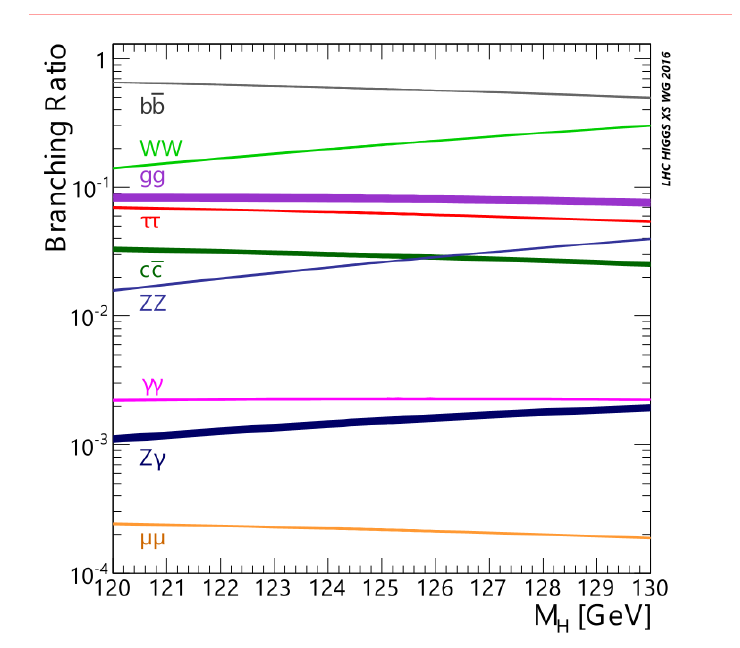
\includegraphics[width=\textwidth]{higgsBranching.PNG}
        \caption{\cite{PhysRevD.98.030001}}
      \end{figure}
    \end{column}
    \begin{column}{0.5\textwidth}
      \begin{itemize}
        \item Relatively high branching ratio
        \vspace{0.3cm}
        \item Hadronically decaying taus are more difficult to select than leptonic ones
      \end{itemize}
    \end{column}
  \end{columns}
\end{frame}


\begin{frame}{\tHq lepditau channel selection}
  \begin{columns}
    \begin{column}{0.5\textwidth}
      \centering 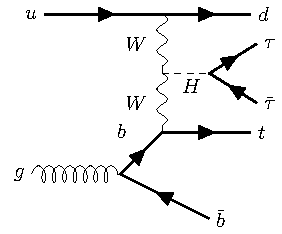
\includegraphics[width=0.7\textwidth]{tHq_tautau}\\
      %\includegraphics[width=0.45\textwidth]{/cephfs/user/s6chkirf/feynman_diagrams/tHq_WW}
      %\includegraphics[width=0.45\textwidth]{/cephfs/user/s6chkirf/feynman_diagrams/tHq_ZZ}
      \begin{itemize}
        \item Number of jets: 2
        \item Number of b-jets: 1
        \item number of leptons: \bf{$1e / \mu$}
        \item number of taus: 2 hadronic taus
        \item $E_{\text{T,miss}}$: no cut (to \SI{800}{GeV})
      \end{itemize}
    \end{column}
    \begin{column}{0.7\textwidth}
      \vspace*{-0.05\textwidth}
      \begin{itemize}
        \item Jets:
        \vspace*{-0.02\textwidth}
        \begin{itemize}
          \item $p_T>\SI{35}{GeV}$
          \item $|\eta|<4.5$
        \end{itemize}
        \item Electrons:
        \vspace*{-0.02\textwidth}
        \begin{itemize}
          \item $p_T>\SI{20}{GeV}$ leading \SI{27}{GeV}
          \item $|\eta|<2.5$ not in 1.37 - 1.52
        \end{itemize}
        \item Muons:
        \vspace*{-0.02\textwidth}
        \begin{itemize}
          \item $p_T>\SI{20}{GeV}$ leading \SI{27}{GeV}
          \item $0.01<|\eta|<2.5$
        \end{itemize}
        \item Taus:
        \vspace*{-0.02\textwidth}
        \begin{itemize}
          \item $p_T>\SI{20}{GeV}$ leading \SI{27}{GeV}
          \item $|\eta|<2.5$ not in 1.37 - 1.52
        \end{itemize}
      \end{itemize}
    \end{column}
  \end{columns}
\end{frame}
  
